\section{Stimuli materials}
\label{sec:expstimulimaterials}

The stimuli materials for the experiment were all generated programmatically by using the Processing 3 software (\url{https://processing.org}), which is based on the Java programming language. The executive files for the generation of the visual stimuli are parametric, meaning that the researchers can input some variables and the software generates a new version of the visual stimuli automatically. For example, all the conversions between pixel and degrees of visual angle measurements units, the drawing of sinusoidal and triangular waves starting from trigonometric parameters, the rendering of the target movement, are automated. This features makes them useful not only for the specific case of the current research on early ASD, but also for other research in need for similar paradigms and visual stimuli.

The eye parameters and the appropriate methods for eliciting them enlisted in the framework (Chapter~\ref{chap:framework}) lead to the development of four kinds of stimuli, which were put together in a single experimental procedure in the SMI Experiment Suite®. In between the presentation of the visual stimuli, a series of interstimulus materials was shown. A summary of the sequence of the visual stimuli and interstimulus materials is shown in Tab.~\ref{tab:stimulisummary}.

\begin{table}[h]
   \centering
   \begin{tabular}{@{}c@{\hspace{.5cm}}c@{}}
       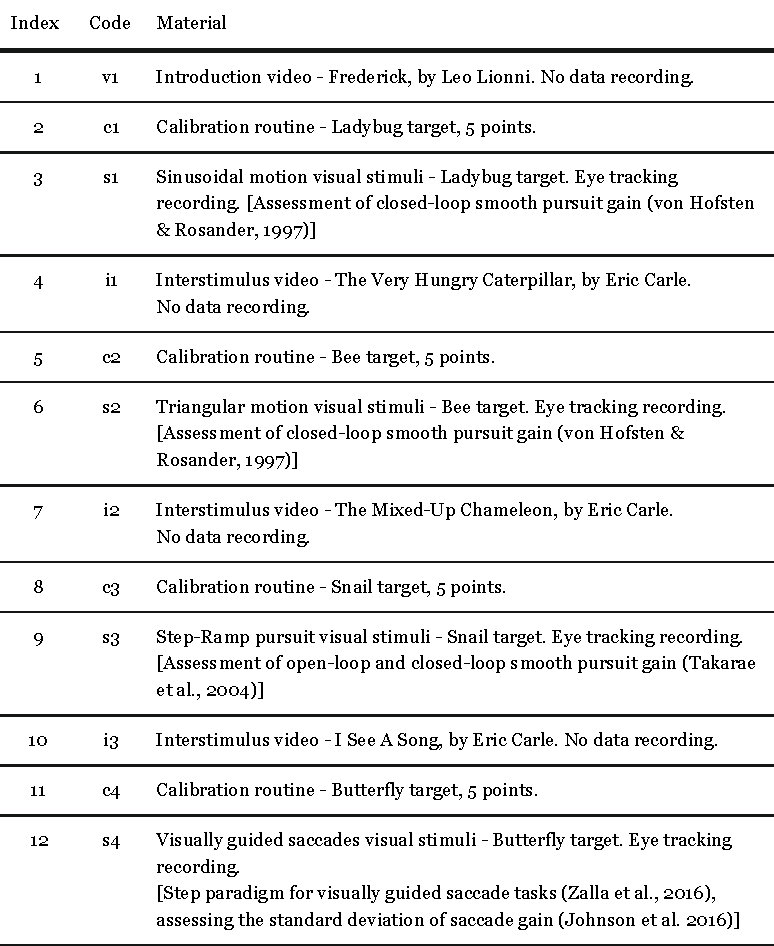
\includegraphics[page=1,width=.8\textwidth]{figures/tables/table_4.pdf}
   \end{tabular}
 \caption{List of stimuli and interstimulus materials.}
 \label{tab:stimulisummary}
\end{table}



\subsection{Stimuli}
\label{sec:expstimuli}

All the stimuli require to input the display monitor sizes and resolution, in order to convert any measurement in pixel units to degrees of visual angle. The degrees of visual angle can be seen as a device-independent measurement unit, therefore it allows to make more precise calculations and to compare the results with literature independently from the type of media on which the stimuli are streamed on. The conversion functions are based on trigonometric calculations made publicly available by Michael Tesar\footnote{The original codes are available at \url{https://github.com/neuropacabra/VisualAngleCalculator}.} and encoded to suit the Processing 3 syntax. For the experiments, the assumed distance of the participant’s eyes from the screen was set to 50 cm.

Given the small size of the display monitor available for doing the experiments, the parameters for the stimuli could not always replicate the stimuli described in literature, which often used supports and media with wider surfaces. Therefore, the stimuli are adapted for being presented on a 15.6” display monitor. Moreover, the parameters for each stimuli (especially the ones related with velocities, repetitions and durations) were manipulated in order to obtain trials short enough to keep the children’s interest throughout the stimuli presentation.

The framerate for the stimuli is set to 60 fps in order to ensure a smooth presentation of the moving target and consequent eye movement artifacts due to a low rendering performance of the stimuli videos. This framerate matched also with the refresh rate of the display monitor used for the experiments.

The target pictures (Fig.~\ref{fig:stimulitargets}) were drawn by the author starting from a black and white version of the ladybug target by Karen Tyler\footnote{The icon is available at \url{https://thenounproject.com/01karent/uploads/?i=469184}.The author made the icon available under creative commons attribuition (CC-BY) license.}. The aspect of the targets (bee, butterfly and snail) was kept consistent, changing their colors in order to make them stand out on the medium-gray background (128 on 256 levels), in the attempt to attract as much attention as possible. The target pictures are the only colored element in the stimuli.

\begin{figure}[h]
  \centering
  
\includegraphics[width=.9\textwidth]{figures/targets-08.jpg}
  \caption[Target pictures for the stimuli]{Target pictures for the stimuli}
  \label{fig:stimulitargets}
\end{figure}

The 5-point calibration routines (c1, c2, c3, c4) used the custom targets, depending on which stimuli they were preceding. The calibration required a precision of \textless 0.5 deg drift to be considered valid. The calibration procedures were semi-automated, for which the researcher needed to input a command in order to start and then the software expected the participant’s fixations on the target to proceed further. The targets were always 49x49 px, covering 1 degree of visual angle for the display monitor in use. This dimension allows the viewers to foveate the whole target \citep[p. 2]{leigh2015neurology}, preventing them to scan inside the target to foveate for further internal details, adding potential intrusive eye movements to the recordings.
The Processing 3 scripts allow to export a picture for each frame in the visual stimuli, and then it can import all the pictures in sequence for creating a movie file. The movie file are then chained together in the eye tracker experiment software.
Each stimulus material has its own set of parameters and algorithms to be generated. Each Processing 3 script generates a report with the parameters for the drawing of the stimuli, in order to allow the researchers to annotate the parameters and confront them within experiments or with literature. The detailed list of the stimuli for each participant is shown in Appendix~\ref{app:stimulidescription}. Here it follows a summary of the algorithms which generate the stimuli.



\subsubsection{Sinusoidal motion visual stimuli [s1, s2]}
\label{sec:expsinestimuli}

These stimuli were drawn starting from the descriptions provided by \cite{vonhofsten1997smoothpursuit}.

Given the limited space available on the 15.6” display monitor, an algorithm for drawing the sinusoidal and triangular motion paths was created in order to exploit all the space available:
\begin{enumerate}
    \item Input the size and the resolution of the screen in pixels;
    \item Convert the size from pixels to degrees of visual angle;
    \item Set the wave parameters:
    \begin{enumerate} [label*=\arabic*.]
        \item Chose the number of cycles per trial (direction). This will impact on the wavelength of the wave;
        \item Set the frequency of the wave (which determines the duration of the trials and the velocity of the wave);
        \item The amplitude by default is set to be half of the display monitor screen;
    \end{enumerate}
    \item Set the number of trials (i.e. the wave completes all the cycles toward one direction) within the experiment
    \item Chose the target picture and its size
    \item Determine the sinusoidal and triangular wave function and use it to move the target. The motion goes from the center-left of the screen to the center-right, and then backwards
\end{enumerate}

The parameters of the waves were made dependent on the number of cycles, in order to allow the researchers to predict how many measurement repetitions could be available from completing all the trials in the visual stimuli.

The frequency of the wave was kept 0.2 Hz, following the values from \cite{vonhofsten1997smoothpursuit}. However, the velocity of the target motion is not comparable with that study, due to the different dimensions of the waves in terms of amplitude and wavelength.

Before starting to move the target in a wave motion, a focusing animation is played for 1 second in order to direct the attention of the participant toward the initial point of the wave.

The two stimuli are essentially the same (Fig.~\ref{fig:sinescreens}, Fig.~\ref{fig:triangscreens}), but they use two different wave equations (sinusoidal sinusoidal $y(x)=Asin(2\pi/\lambda*x) $ ; triangular $y(x)=2A/\pi*arcsin(sin(2\pi/\lambda*x)$)) and different target pictures.

\begin{figure}[h]
  \centering
  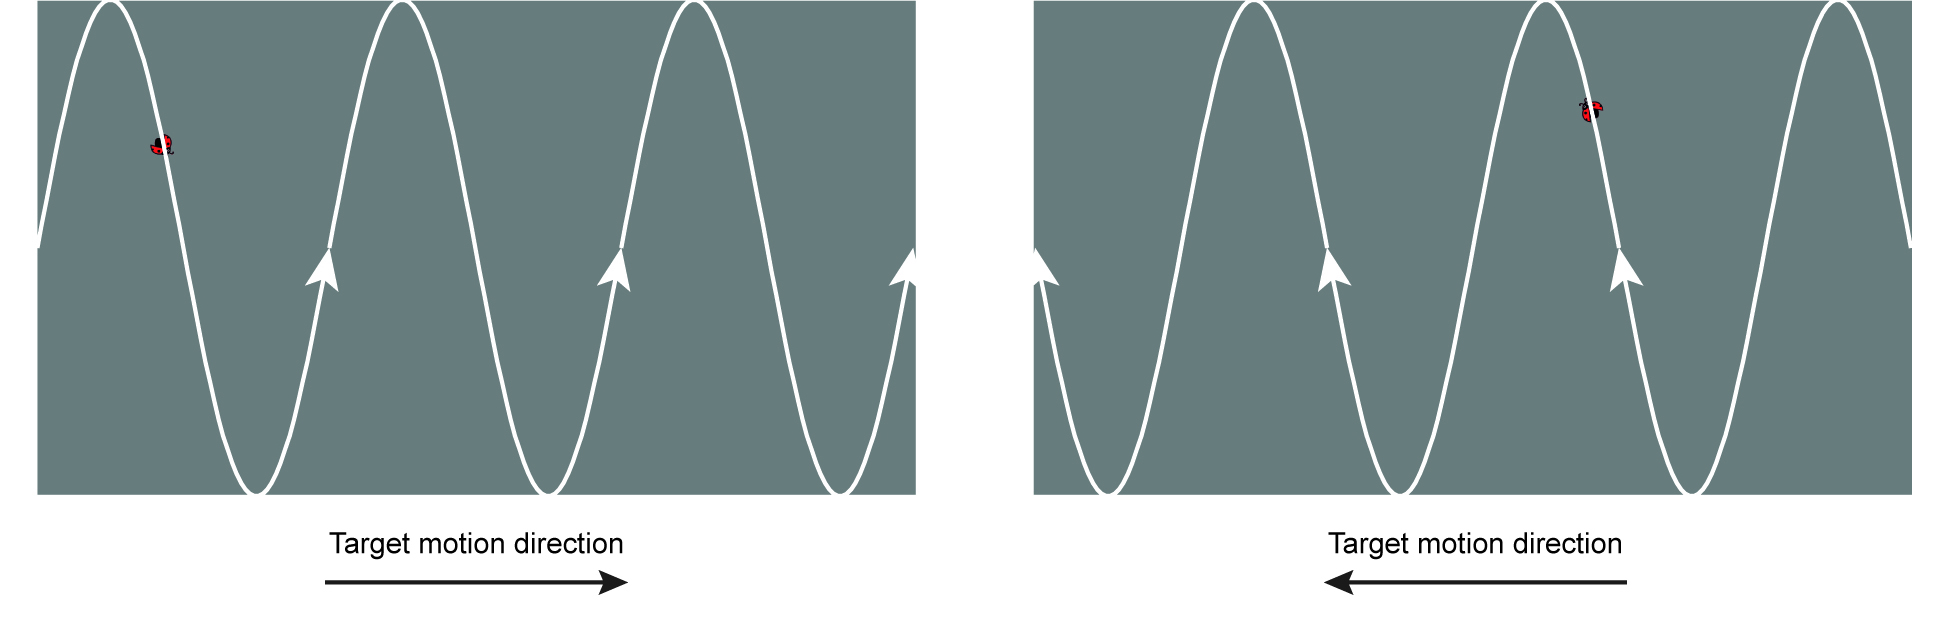
\includegraphics[width=.9\textwidth]{figures/stimulitarget-09.jpg}
  \caption[Sinusoidal stimuli screenshots]{Scheme of the sinusoidal motion stimuli (s1)}
  \label{fig:sinescreens}
\end{figure}

\begin{figure}[h]
  \centering
  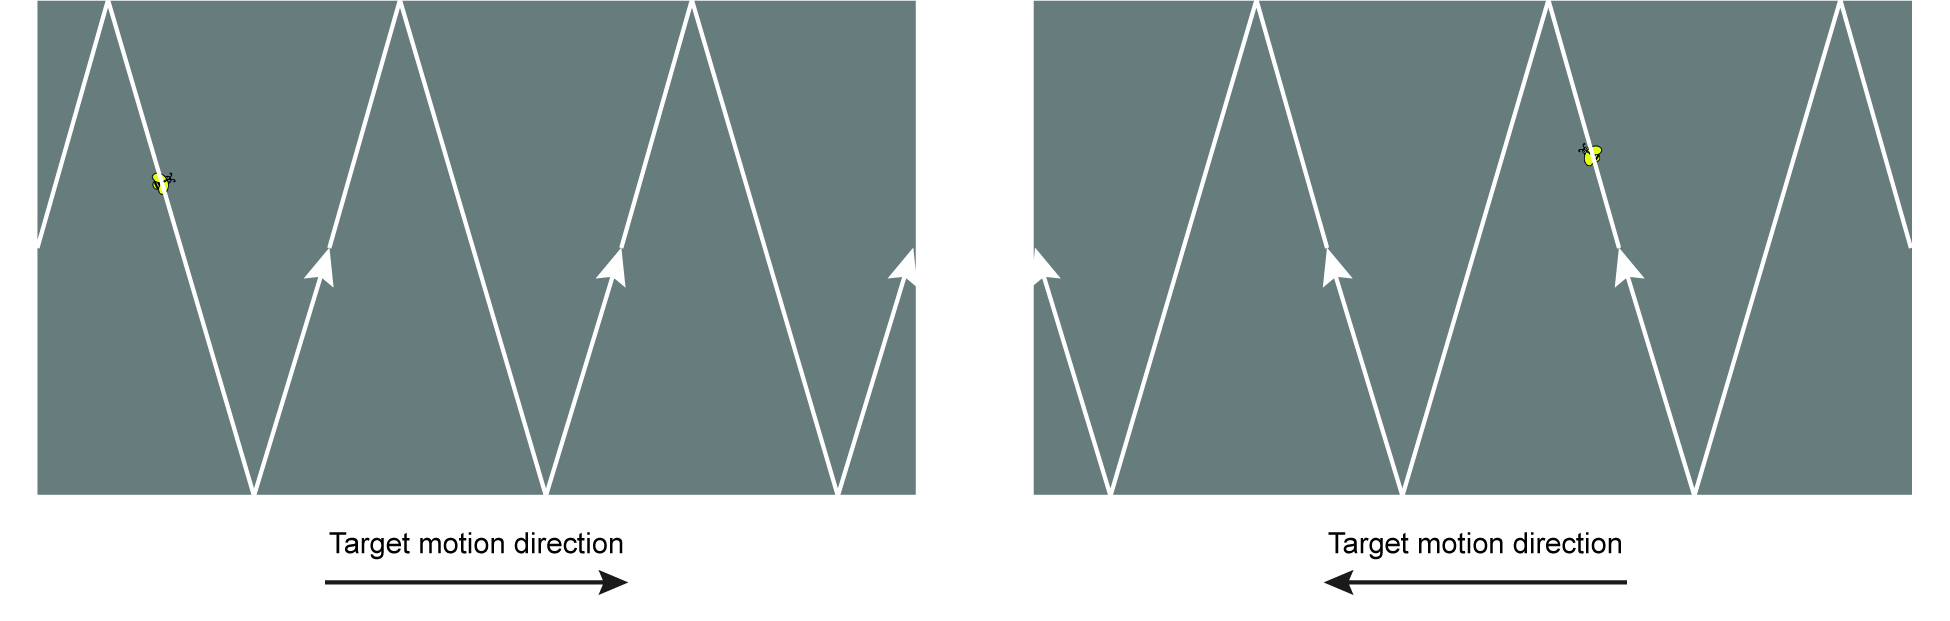
\includegraphics[width=.9\textwidth]{figures/stimulitarget-10.jpg}
  \caption[Triangular stimuli screenshots]{Scheme of the triangular motion stimuli (s2)}
  \label{fig:triangscreens}
\end{figure}




\subsubsection{Step-Ramp pursuit visual stimuli [s3]}
\label{sec:expstepramp}

The algorithm for drawing a target moving smoothly following a step-ramp paradigm (Fig.~\ref{fig:steprampscreens}) was taken from \cite{takarae2004smoothpursuit}:
\begin{enumerate}
    \item Show the central target for a random interval of time between two extremes: 1 s and 2 s. The randomization helps in preventing anticipatory eye movements.
    \item Move the target abruptly to a determined distance but random direction on the horizontal axis:
    \begin{enumerate}[label*=\arabic*.]
        \item 3 deg of visual angle
        \item either left or right
    \end{enumerate}
    \item Smooth movement of the target, at a constant but randomized velocity value, from the step position to a second position, keeping the same direction of the step:
    \begin{enumerate}[label*=\arabic*.]
        \item from 3 to 15 deg of visual angle
        \item at two different velocities: 4 and 8 degrees/second
        \item in two different directions: either left or right depending on the step direction
    \end{enumerate}
    \item When the target reaches the final position, start another trial. Repeat the trial for each velocity by a set amount of times: 2 trials for each velocity.
\end{enumerate}

The Processing 3 code generates an array with all the velocity and direction profiles, then it shuffles the array in order to have always a randomized sequence. This is the only experiment in which the orientation of the target matters. Therefore the snail target turns toward the direction of the movement on each trial.

\begin{figure}[h]
  \centering
  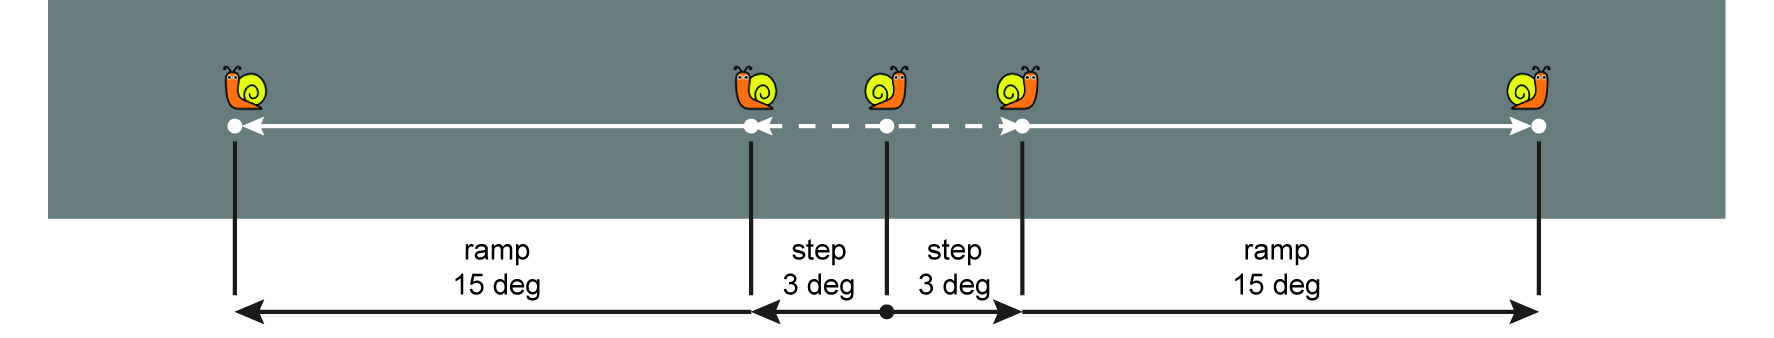
\includegraphics[width=.9\textwidth]{figures/stimulitarget-11.jpg}
  \caption[Step-ramp stimuli screenshots]{Scheme for of the step-ramp stimuli (s3)}
  \label{fig:steprampscreens}
\end{figure}



\subsubsection{Visually guided saccades visual stimuli [s4]}
\label{sec:expsaccades}

The algorithm for drawing a moving target in space following a step paradigm (Fig.~\ref{fig:saccadescreens}) was taken from \cite{zalla2016saccades}:
\begin{enumerate}
    \item Show the central target for a random interval of time between two extremes: 1 s and 2 s. The randomization helps in preventing anticipatory eye movements.
    \item At the same time, hide the central target and show a peripheral target, at a random distance between two extremes, in a random direction:
    \begin{enumerate}[label*=\arabic*.]
        \item the peripheral target is shown for a random interval of time between 1 s and 2 s
        \item in two different directions: either left or right (50-50 proportion)
        \item between 5 to 15 degrees of visual angle. The script randomizes both the x and y coordinates of the peripheral target, even if the guidelines did not explicitly state if the random y was needed. However, if the peripheral target always appears at y=0 (horizontal axis), some prediction mechanism could arise in the subject, who most likely understands after a couple of trials that the target would appear at the same y coordinate. In order to avoid this kind of prediction, the targets are both moved left or right from the central target at a random degree of visual angle in the range 5-15 deg, and also rotated around the central point of a random degree between +45 deg and -45 deg from the horizontal axis (not more, in order to retain the perception horizontal movement direction). 
    \end{enumerate}
    \item When the peripheral target disappear, start another trial. Repeat the trial for a set amount of times: 15 times.
\end{enumerate}

The Processing 3 code generates an array with all the distance and direction profiles, then it shuffles the array in order to have always a randomized sequence.

The number of repetitions was 15, in order to have a total length of the trial ranging from 30 s to 60 s. \cite{smyrnis2008guidelines} advices to have at least 30 repetitions, however in that case the trial would range between 60 to 120 s, which was considered a too long timeframe for a small child for sustaining the attention. Indeed, in this last part of the experiment, the children shown less attention span to the stimuli.

\begin{figure}[h]
  \centering
  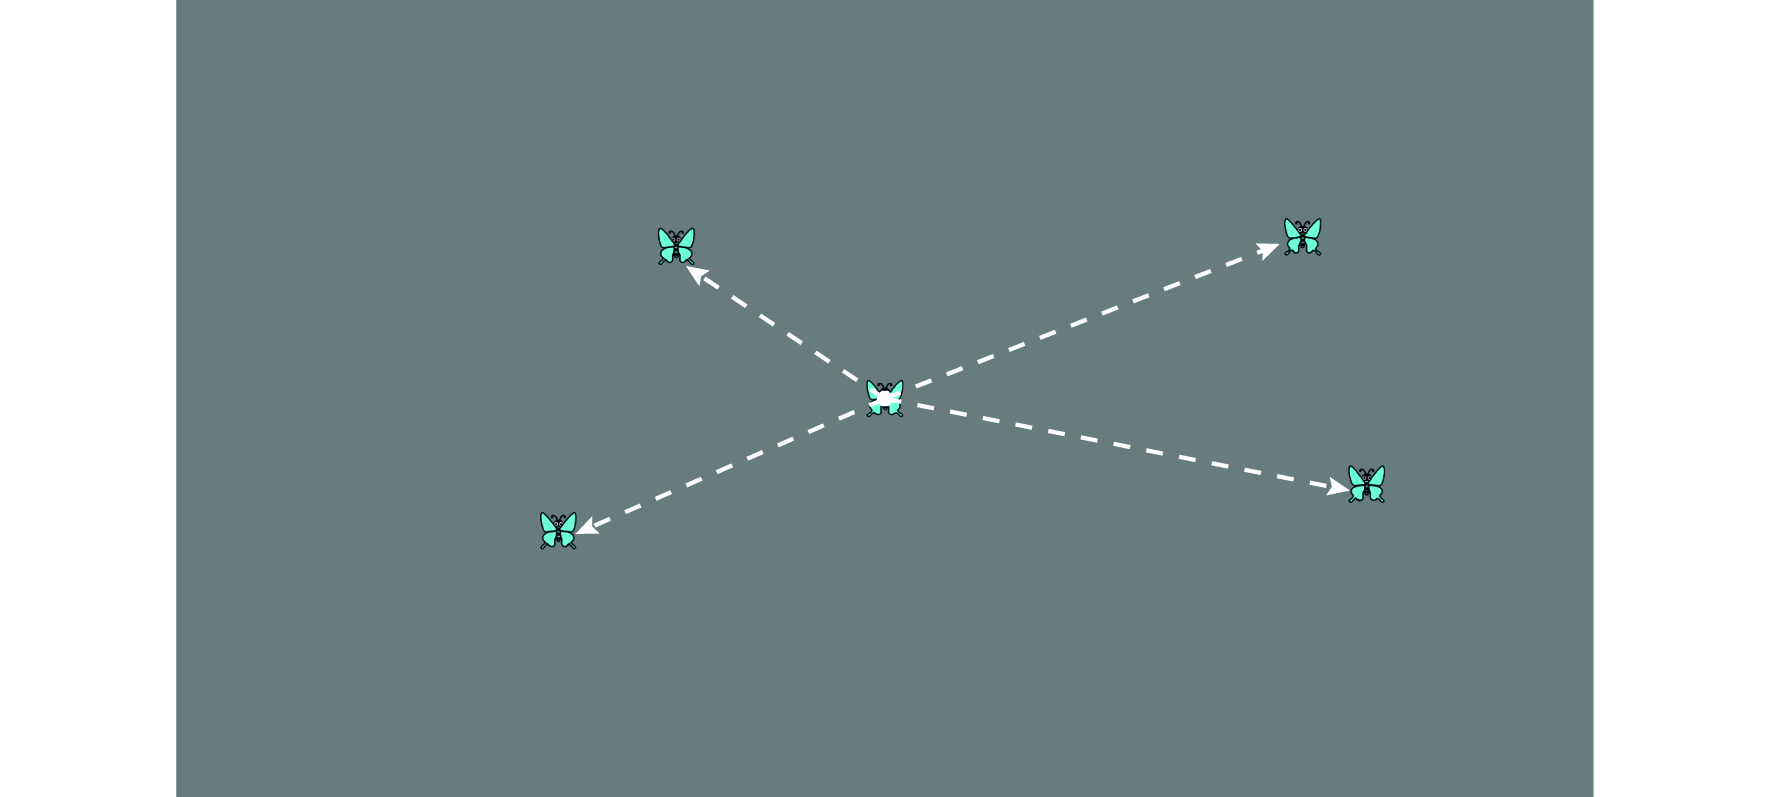
\includegraphics[width=.8\textwidth]{figures/stimulitarget-12.jpg}
  \caption[Saccade stimuli screenshots]{Scheme of the saccade stimuli (s4)}
  \label{fig:saccadescreens}
\end{figure}

\subsection{Interstimulus materials}
\label{sec:expinterstimulus}

The interstimulus materials chosen for the experimentation are a series of videos, which shown animations and storytelling based on famous books for small children: “Frederick” by Leo Lionni, and “The Very Hungry Caterpillar”, “The Mixed-Up Chameleon” and “ I See A Song” by Eric Carle. All the videos are publicly available on the Youtube website. These animations were chosen due to the fact that they are based on stories made for being appropriate for small children and pretty renown internationally for their good contents, and above all they are not frightening or stressing the child in any way. The function of the interstimulus materials is indeed to provide a break in between the stimuli presentation. While the interstimulus videos are shown, the eye tracker does not record data. This can be seen as a potential data loss, due to the fact that analyzing the gaze patterns of the children while they watch the animations can be a source of valuable information. However, the priority in this experimentation was given to the opportunity for the children and their caregivers to relax, have playful stress-relieving activities and granting them freedom of movement. The automatic calibration routines shown after the interstimulus materials correct any possible calibration drift.

Moreover, a specific experimental design should be created around the interstimulus videos if they would be considered experimental stimuli. This task goes beyond the scope of the current research.
During the experiment session, it was not necessary to show the first video, “Frederick” by Leo Lionni. The children and their caregivers were already ready to start, and the children were showing interest for the experiment computer. Therefore the experiments started with the first calibration routine right away.

The duration of the interstimulus videos was planned to be around 2 minutes. However during the experiments it become evident that this amount of time was too long, and it distracted the children probably too much. They started losing interest after around 1 minute. However, all the animations showed an introduction, which does not present any animated contents but just texts. Probably it could have been more useful to skip systematically the introduction parts and show shorter parts of animated contents right away.
